\chapter{Observability and metrics}
\label{chap:osservabilita}

\section{Publishing the metrics}

Operational metrics can typically reach whoever observes them in two ways: either someone else
periodically queries every service (\emph{pull}), or every service sends them on its own
initiative (\emph{push}).
RAM-USB adopts the second: every service publishes its own metrics once a minute,
on its own dedicated MQTT topic to the Mosquitto broker \cite{mosquitto-github}.
The choice stems from the fact that a \emph{pull} model would require Metrics-Collector to open a
connection to each of the six services, widening the mesh reachability rules discussed in
\autoref{chap:rete}.
Because the services publish on their own initiative, they are instead the ones that open the connection to the broker.
From there, Metrics-Collector reads the metrics and persists them in a database.

Operational metrics do not contain user data, but the system's metadata must be protected with the
same care; for this reason the communications take place inside the private network and are protected by mTLS,
with certificates issued by the internal CA.

Every publication carries as its body a six-field payload, shown in \autoref{lst:metrics-payload}.
The metrics in the payload refer to the minute in which they were sent.

\Needspace{10\baselineskip}
\begin{lstlisting}[caption={Structure of the metrics payload, from \texttt{payload.go}
\cite{ramusb-code-metrics-payload}.}, label={lst:metrics-payload}]
type Payload struct {
	Service               string  `json:"service"`
	Timestamp             string  `json:"timestamp"`
	RequestCount          int64   `json:"request_count"`
	ErrorCount            int64   `json:"error_count"`
	AverageResponseTimeMs float64 `json:"average_response_time_ms"` 
	ActiveConnections     int64   `json:"active_connections"`
}
\end{lstlisting}

The publications all use \emph{QoS 1} (at least once), in the MQTT classification \cite{oasis-mqtt-311}: the
broker guarantees that the message arrives at least once, at the cost of a possible duplicate. \emph{QoS 0}
(at most once) is ruled out because RAM-USB cannot afford to lose metrics silently; \emph{QoS 2}
(exactly once) is ruled out because the extra guarantee it offers (the absence of duplicates) is not needed here,
since a duplicate only results in two overlapping points at the same instant, invisible on the
chart.

\section{Reception and consistency check}

The published message must reach a single recipient. This property is enforced
by the Mosquitto ACL, which ensures that every service can only write to its own topic, while
Metrics-Collector can read from the \texttt{metrics/\#} topics without being able to write to them.

That ACL, however, does not prevent a compromised service, while staying within its own legitimate write
permission, from publishing a payload whose declared \texttt{service} field is a name different from
its own.
Metrics-Collector therefore revalidates every message independently, deriving the expected
service from the topic the message arrived on and comparing it with the one declared in the payload.
On any discrepancy it discards the message and records it in the logs.

\section{Time-series persistence}

Metrics-Collector persists the metrics in TimescaleDB \cite{timescaledb-github}, an extension of
PostgreSQL designed for a workload made almost entirely of time-ordered writes.

The \texttt{metrics} table has no primary key, since a row of metrics has no natural
identity. Moreover, TimescaleDB \cite{timescaledb-github} does not require one. It is organized in chunks by
time intervals on the \texttt{time} column: the two background policies in
\autoref{lst:metrics-policies} act chunk by chunk, based on their age. The first drops every chunk
older than thirty days; the second, after seven days, moves the chunks into a compressed columnar
format, grouped by service and ordered by descending time.

\Needspace{18\baselineskip}
\begin{lstlisting}[language=sql, caption={Automatic retention and compression policies of the
\texttt{metrics} table, from \texttt{000001\_create\_metrics\_table.up.sql} \cite{ramusb-code-metrics-schema}.},
label={lst:metrics-policies}]
SELECT create_hypertable('metrics', by_range('time'));

SELECT add_retention_policy('metrics', drop_after => INTERVAL '30 days');

ALTER TABLE metrics SET (
	timescaledb.enable_columnstore,
	timescaledb.segmentby = 'service',
	timescaledb.orderby = 'time DESC'
);
CALL add_columnstore_policy('metrics', after => INTERVAL '7 days');
\end{lstlisting}

\section{Metrics visualization}

An administrator checks the health of the system, without that consultation
ever touching the users' data since, by construction, the metrics do not contain any.
Grafana \cite{grafana-github} reads from TimescaleDB directly.

To contact TimescaleDB, in addition to reachability on the mesh network and Grafana's mTLS certificate,
a password is also required, following the same defense-in-depth principle already seen for Headscale's
administrative API in \autoref{chap:rete}.

The dashboard shows three panels, each a direct query on the \texttt{metrics} table: average
response time, throughput, and active connections.

\autoref{fig:metrics-flow} summarizes the entire pipeline just described, from publication on the MQTT
topic to the dashboard.

\begin{figure}[H]
    \centering
    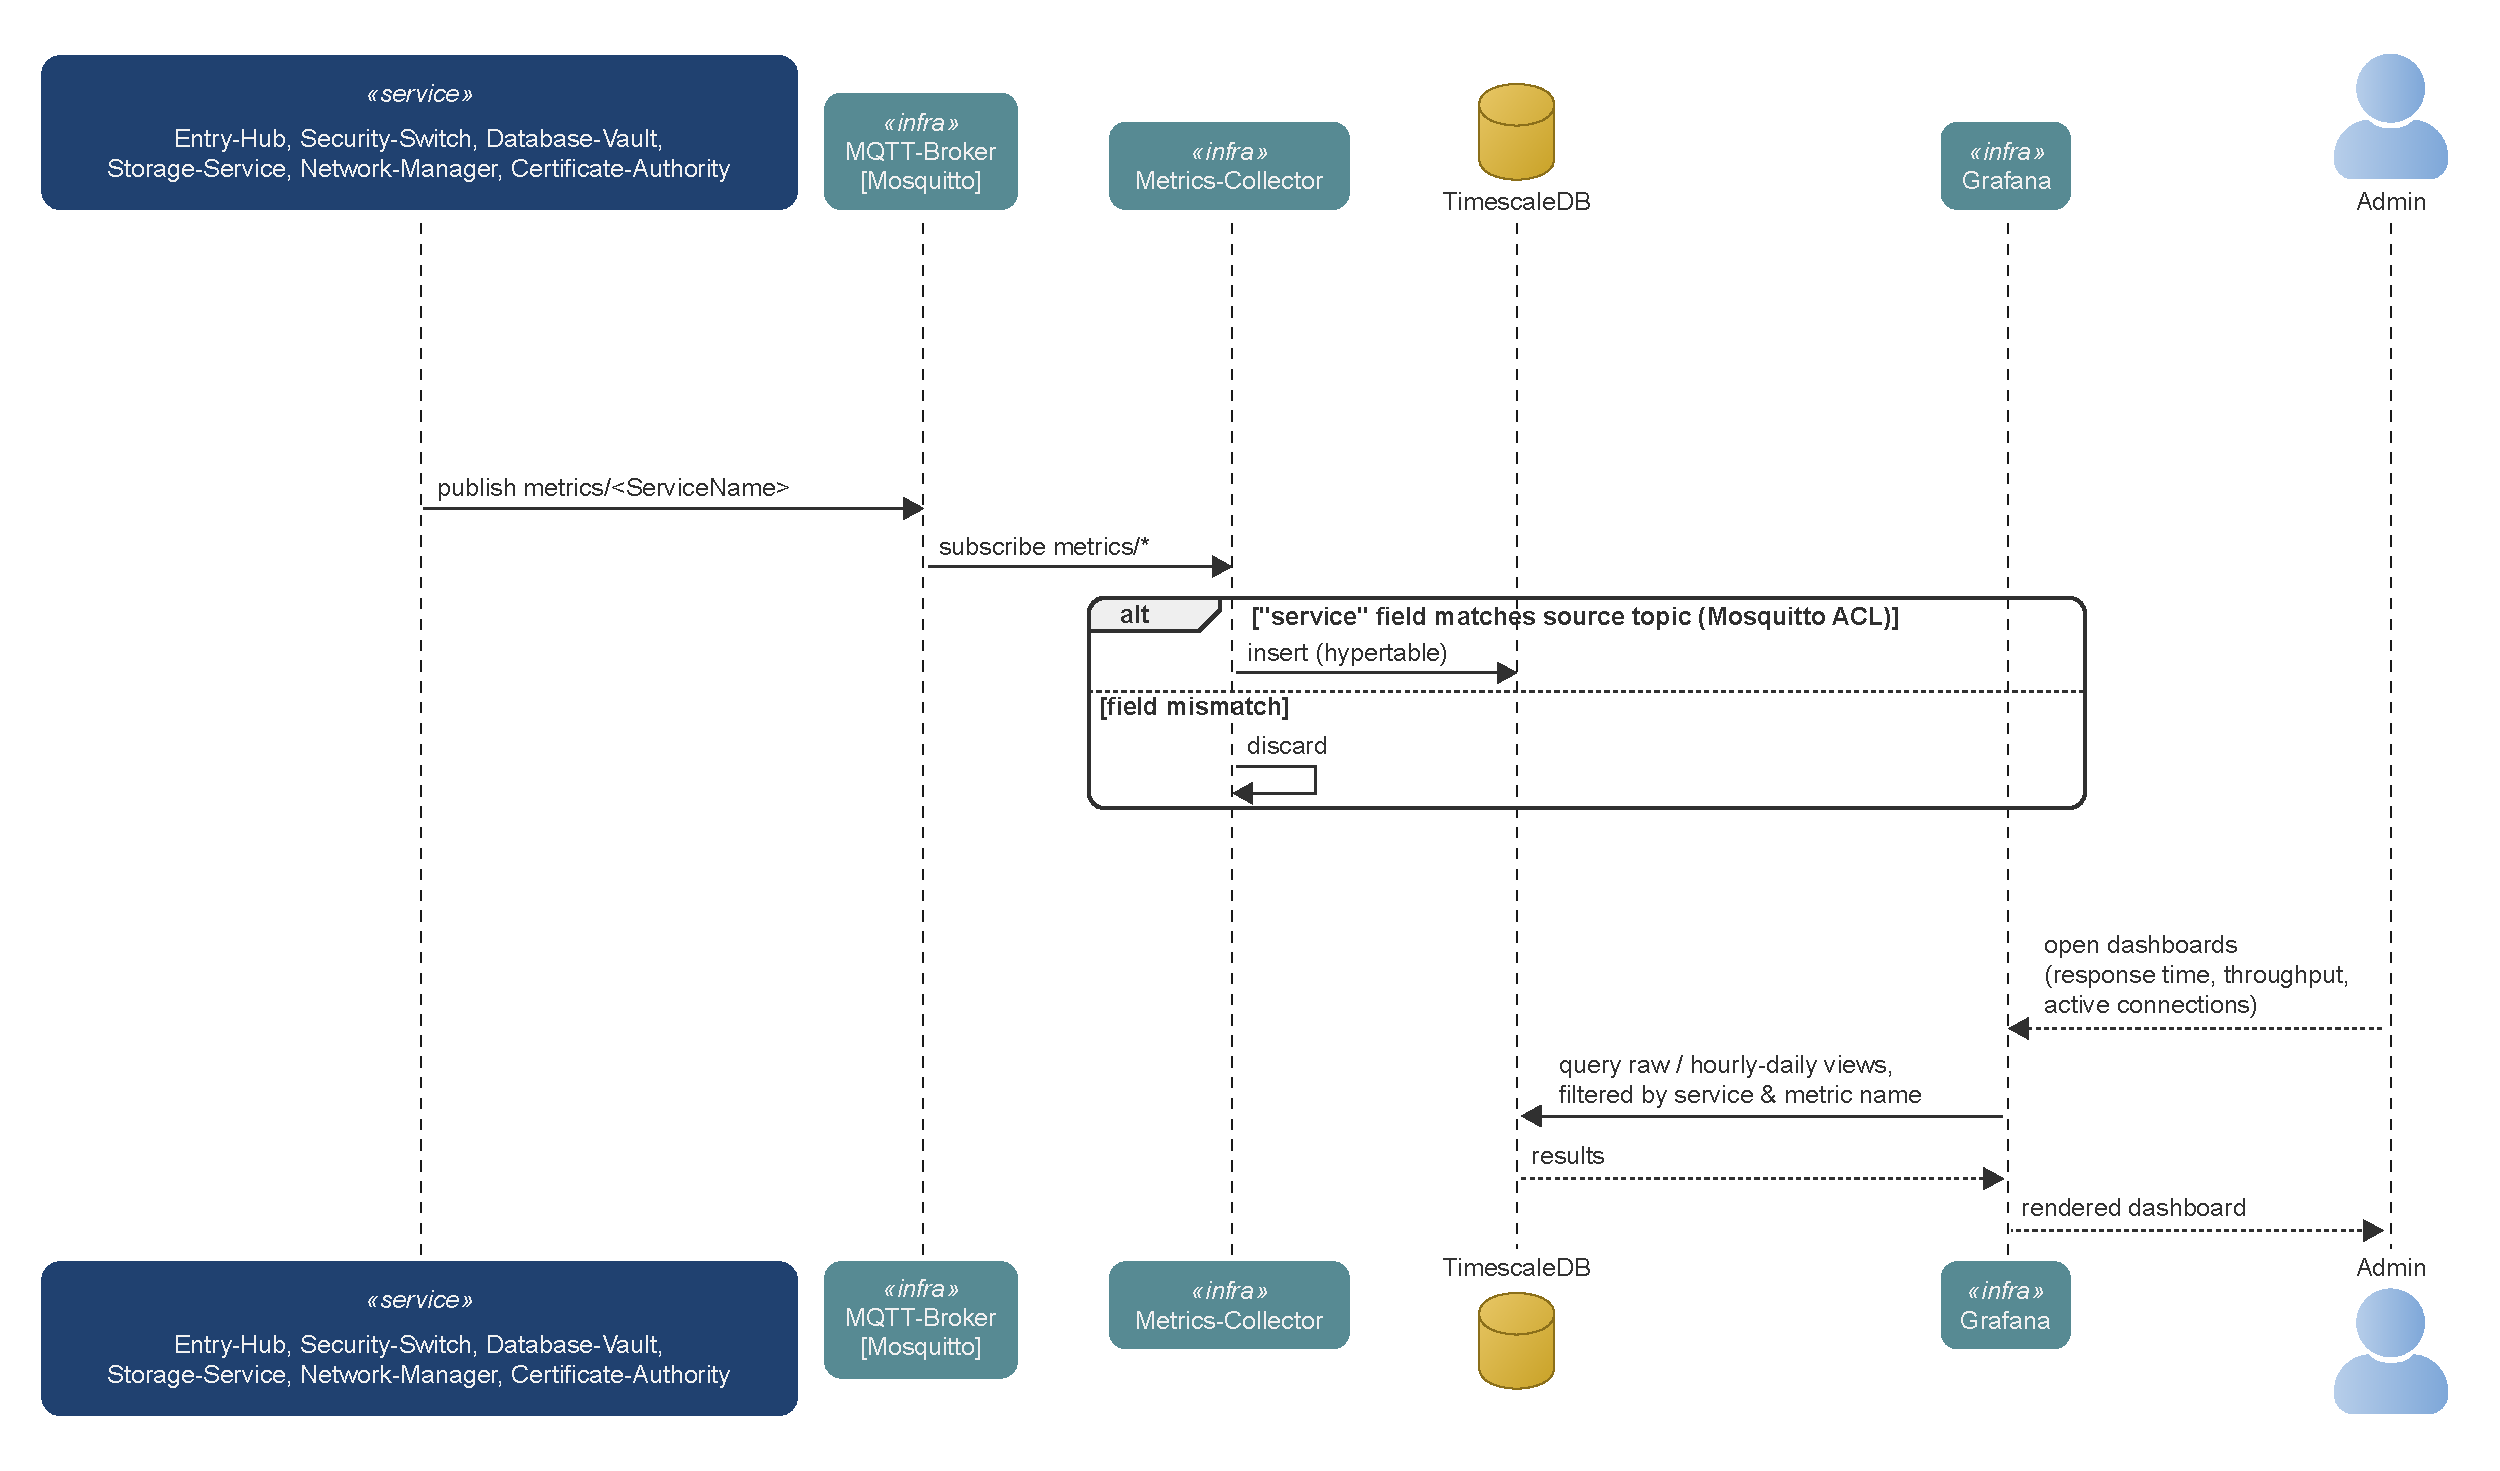
\includegraphics[width=\textwidth]{figures/11-operations-metrics-flow.pdf}
    \caption{Observability pipeline, from the publication of the metrics to the Grafana dashboard.}
    \label{fig:metrics-flow}
\end{figure}
